% Candidate source: src-e83c48821eaac4546df1607aa7bd47f8c49362fe9d091f3ff8accf356722e61c
% Source PDF SHA-256: 0a787b530b939cb104a802de2c27119b5d150bac7c4f0e78b069bc103f381232
% PDF page 1 (printed page 206), question 11.
% Redraw follows visible relations: derivative graph y = f'(x) and four candidate curves (A)–(D).
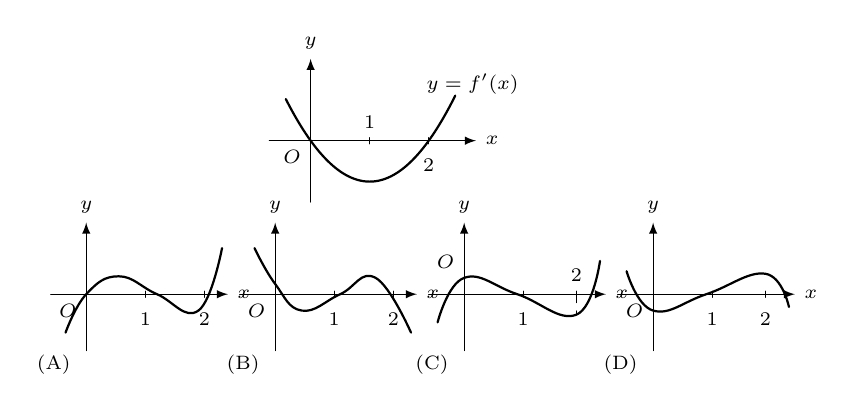
\begin{tikzpicture}[line cap=round,line join=round,>=latex,x=0.75cm,y=0.65cm,every node/.style={font=\scriptsize}]
  % Top: prompt curve y = f'(x)
  \begin{scope}[shift={(3.8,3.0)}]
    \draw[->] (-0.7,0) -- (2.8,0) node[right] {$x$};
    \draw[->] (0,-1.2) -- (0,1.6) node[above] {$y$};
    \node[below left] at (0,0) {$O$};
    \draw[thick,domain=-0.42:2.45,samples=80] plot (\x,{0.8*\x*(\x-2)});
    \draw (1,0.06) -- (1,-0.06) node[above=2pt] {$1$};
    \draw (2,0.06) -- (2,-0.06) node[below=2pt] {$2$};
    \node[right] at (1.8,1.1) {$y = f'(x)$};
  \end{scope}

  % Bottom: Four candidate graphs (A), (B), (C), (D)
  % (A)
  \begin{scope}[shift={(0,0)}]
    \draw[->] (-0.6,0) -- (2.4,0) node[right] {$x$};
    \draw[->] (0,-1.1) -- (0,1.4) node[above] {$y$};
    \node[below left] at (0,0) {$O$};
    \draw[thick] plot[smooth,tension=0.75] coordinates {(-0.35,-0.75) (0,0) (0.55,0.35) (1.2,0) (1.9,-0.32) (2.3,0.9)};
    \draw (1,0.06) -- (1,-0.06) node[below=2pt] {$1$};
    \draw (2,0.06) -- (2,-0.06) node[below=2pt] {$2$};
    \node[below left] at (-0.1,-1.0) {(A)};
  \end{scope}

  % (B)
  \begin{scope}[shift={(3.2,0)}]
    \draw[->] (-0.6,0) -- (2.4,0) node[right] {$x$};
    \draw[->] (0,-1.1) -- (0,1.4) node[above] {$y$};
    \node[below left] at (0,0) {$O$};
    \draw[thick] plot[smooth,tension=0.75] coordinates {(-0.35,0.9) (0,0.2) (0.45,-0.32) (1.1,0) (1.7,0.32) (2.3,-0.75)};
    \draw (1,0.06) -- (1,-0.06) node[below=2pt] {$1$};
    \draw (2,0.06) -- (2,-0.06) node[below=2pt] {$2$};
    \node[below left] at (-0.1,-1.0) {(B)};
  \end{scope}

  % (C) - Correct option
  \begin{scope}[shift={(6.4,0)}]
    \draw[->] (-0.6,0) -- (2.4,0) node[right] {$x$};
    \draw[->] (0,-1.1) -- (0,1.4) node[above] {$y$};
    \node[above left] at (0,0.32) {$O$};
    \draw[thick] plot[smooth,tension=0.75] coordinates {(-0.45,-0.55) (0,0.32) (0.9,0) (1.9,-0.4) (2.3,0.65)};
    \draw[dashed] (1.9,0) -- (1.9,-0.4);
    \draw (1,0.06) -- (1,-0.06) node[below=2pt] {$1$};
    \draw (1.9,0.06) -- (1.9,-0.06) node[above=2pt] {$2$};
    \node[below left] at (-0.1,-1.0) {(C)};
  \end{scope}

  % (D)
  \begin{scope}[shift={(9.6,0)}]
    \draw[->] (-0.6,0) -- (2.4,0) node[right] {$x$};
    \draw[->] (0,-1.1) -- (0,1.4) node[above] {$y$};
    \node[below left] at (0,0) {$O$};
    \draw[thick] plot[smooth,tension=0.75] coordinates {(-0.45,0.45) (0,-0.32) (0.9,0) (1.9,0.4) (2.3,-0.25)};
    \draw (1,0.06) -- (1,-0.06) node[below=2pt] {$1$};
    \draw (1.9,0.06) -- (1.9,-0.06) node[below=2pt] {$2$};
    \node[below left] at (-0.1,-1.0) {(D)};
  \end{scope}
\end{tikzpicture}
